\documentclass[12pt]{article}

\usepackage[margin=1in]{geometry}
\usepackage{graphicx}
\usepackage{booktabs}
\usepackage{hyperref}
\usepackage{listings}
\usepackage{xcolor}
\usepackage{amsmath}
\usepackage{tikz}
\usetikzlibrary{arrows.meta, positioning, shapes.geometric}

\hypersetup{
    colorlinks=true,
    linkcolor=blue,
    urlcolor=blue,
    citecolor=blue
}

\lstset{
    basicstyle=\ttfamily\small,
    backgroundcolor=\color{gray!10},
    frame=single,
    breaklines=true,
    columns=fullflexible
}

\title{Conversation-to-Calendar AI\\[0.5em]
\large System Architecture \& Performance Report}
\author{}
\date{March 2026}

\begin{document}

\maketitle
\tableofcontents
\newpage

% ============================================================
\section{Introduction}

This document describes the architecture and performance of the
Conversation-to-Calendar AI system---a demonstration pipeline that ingests
natural-language conversation transcripts with speaker labels and
automatically creates, updates, or deletes events on the owner's Google
Calendar using LLM-driven extraction.

The system is built with Python~3.12, Google Gemini~2.5~Pro for
intelligence, and the Google Calendar API for calendar operations. It is
packaged as a Docker container with a web frontend for interactive use.

% ============================================================
\section{System Architecture}

\subsection{Design Philosophy}

The architecture prioritizes \textbf{observability over autonomy}. Rather
than giving the LLM direct access to the calendar API (an agentic
approach), the pipeline separates concerns: the LLM outputs structured
JSON describing desired calendar actions, and Python code validates,
dispatches, and logs each operation. This enables clear inspection of AI
reasoning before any side effects occur.

Every stage degrades gracefully---failure in memory loading, calendar
context fetching, or memory writing logs a warning but does not block the
pipeline. Only a complete extraction failure (Stage~2) results in zero
events processed.

\subsection{Pipeline Overview}

The pipeline executes five sequential stages:

\begin{center}
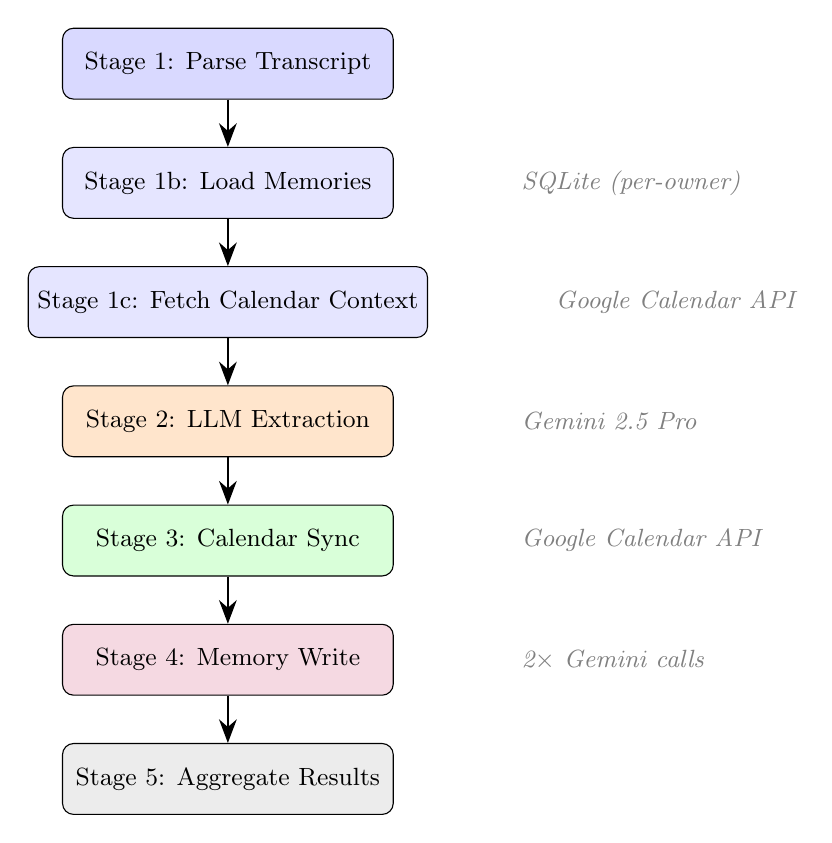
\begin{tikzpicture}[
    stage/.style={draw, rounded corners, minimum width=4.2cm,
                  minimum height=0.9cm, align=center, font=\small},
    arrow/.style={-{Stealth[length=3mm]}, thick},
    node distance=0.6cm
]
\node[stage, fill=blue!15]   (s1)  {Stage 1: Parse Transcript};
\node[stage, fill=blue!10, below=of s1]  (s1b) {Stage 1b: Load Memories};
\node[stage, fill=blue!10, below=of s1b] (s1c) {Stage 1c: Fetch Calendar Context};
\node[stage, fill=orange!20, below=of s1c] (s2)  {Stage 2: LLM Extraction};
\node[stage, fill=green!15, below=of s2]  (s3)  {Stage 3: Calendar Sync};
\node[stage, fill=purple!15, below=of s3] (s4)  {Stage 4: Memory Write};
\node[stage, fill=gray!15, below=of s4]   (s5)  {Stage 5: Aggregate Results};

\draw[arrow] (s1) -- (s1b);
\draw[arrow] (s1b) -- (s1c);
\draw[arrow] (s1c) -- (s2);
\draw[arrow] (s2) -- (s3);
\draw[arrow] (s3) -- (s4);
\draw[arrow] (s4) -- (s5);

\node[right=1.5cm of s1b, font=\small\itshape, text=gray] {SQLite (per-owner)};
\node[right=1.5cm of s1c, font=\small\itshape, text=gray] {Google Calendar API};
\node[right=1.5cm of s2,  font=\small\itshape, text=gray] {Gemini 2.5 Pro};
\node[right=1.5cm of s3,  font=\small\itshape, text=gray] {Google Calendar API};
\node[right=1.5cm of s4,  font=\small\itshape, text=gray] {2$\times$ Gemini calls};
\end{tikzpicture}
\end{center}

\subsection{Stage Descriptions}

\paragraph{Stage 1: Parse Transcript.}
Reads a \texttt{.txt} file with the format \texttt{[Speaker Name]: dialogue text}.
Extracts unique speakers and utterances; validates UTF-8 encoding.

\paragraph{Stage 1b: Load Memories.}
Opens a per-owner SQLite database and loads stored scheduling facts grouped
into five categories: \emph{preferences}, \emph{people}, \emph{vocabulary},
\emph{patterns}, and \emph{corrections}. These are formatted and injected
into the LLM system prompt.

\paragraph{Stage 1c: Fetch Calendar Context.}
Retrieves the owner's upcoming 14~days of calendar events via the Google
Calendar API. Event IDs are remapped from 36-character UUIDs to sequential
integers (1, 2, 3, \ldots) to reduce LLM error rates (from $\sim$50\%
with UUIDs to $\sim$5\% with integers). The formatted context is appended
to the system prompt.

\paragraph{Stage 2: LLM Extraction.}
The core intelligence stage. Gemini~2.5~Pro receives the transcript along
with memory and calendar context, and outputs structured JSON describing
calendar actions (\texttt{create}, \texttt{update}, or \texttt{delete})
with fields for title, times, location, attendees, confidence, and
reasoning.

\paragraph{Stage 3: Calendar Sync.}
For each extracted event, the sync dispatcher validates the data and
executes the appropriate Google Calendar API call. Updates and deletes
with a matched \texttt{existing\_event\_id} use direct API calls; on
HTTP~404 (event deleted since context was fetched), updates fall back to
create and deletes are treated as idempotent success.

\paragraph{Stage 4: Memory Write.}
A dual-call architecture using two sequential Gemini calls:
\begin{enumerate}
    \item \textbf{Fact extraction}---identifies scheduling-relevant facts
          from the transcript (e.g., ``Alice prefers morning meetings'').
    \item \textbf{Action decision}---compares candidate facts against
          existing memories and decides ADD, UPDATE, DELETE, or NOOP.
\end{enumerate}
All operations are logged to an audit table.

\paragraph{Stage 5: Aggregate Results.}
Collects timing, token usage, sync outcomes, and warnings into a final
\texttt{PipelineResult}.

\subsection{Memory System}

The memory system provides persistent, per-owner storage of
scheduling-relevant facts using SQLite with WAL mode. Each owner gets an
isolated database file (e.g., \texttt{data/memory\_alice\_smith.db}).

Memories are organized into five categories:

\begin{center}
\begin{tabular}{@{}ll@{}}
\toprule
\textbf{Category} & \textbf{Example} \\
\midrule
preferences & ``Alice prefers morning meetings (before 11am)'' \\
people      & ``Bob is Alice's manager; weekly 1:1 on Tuesdays'' \\
vocabulary  & ``Wellness hour = therapy appointment'' \\
patterns    & ``Standup is always 15 minutes'' \\
corrections & ``Standup is 15 min, not 30 (corrected)'' \\
\bottomrule
\end{tabular}
\end{center}

The read path injects memories into the LLM prompt before calendar
context. The write path extracts new facts and reconciles them with
existing memories after each pipeline run. Both paths degrade gracefully
on failure.

\subsection{Web Frontend}

The web frontend uses FastAPI with Jinja2 templates and vanilla
JavaScript. The pipeline page provides a split-view interface: transcript
input on the left, real-time pipeline progress on the right via
Server-Sent Events (SSE). A memory viewer page displays stored facts in
an accordion layout grouped by category.

An \texttt{asyncio.Lock} prevents overlapping pipeline runs, returning
HTTP~409 if a second request arrives while one is in progress.

\subsection{Deployment}

The system is containerized with Docker (Python~3.12-slim base). The
default command starts the web server on port~8000. Environment variables
(\texttt{GEMINI\_API\_KEY}, \texttt{GOOGLE\_ACCOUNT\_EMAIL},
\texttt{OWNER\_NAME}) are passed via \texttt{.env}.

% ============================================================
\section{Prompt Engineering \& Fine-Tuning}

\subsection{Prompt Structure}

The system prompt is over 450~lines and includes:

\begin{itemize}
    \item \textbf{Role framing}---extract events for a specific owner from
          their perspective.
    \item \textbf{Current datetime}---injected at inference time for
          resolving relative time references (``tomorrow'', ``next Thursday'').
    \item \textbf{14 filtering rules}---explicit instructions on what
          \emph{not} to extract (sarcasm, past tense, hypotheticals,
          negation, retracted proposals, unmet preconditions, etc.).
    \item \textbf{CRUD decision rules}---when to create, update, or delete,
          with asymmetric confidence thresholds (create: medium OK;
          update/delete: high only).
    \item \textbf{11 title formatting rules}---professional calendar-style
          naming conventions.
    \item \textbf{Few-shot examples}---4~positive and 6~negative
          counter-examples.
    \item \textbf{Dynamic context}---memory facts and calendar events
          injected at runtime.
\end{itemize}

\subsection{Iteration Process}

Prompt engineering followed a structured train/validation split approach
across 13~iterations (runs 0--12). The test suite was divided into:

\begin{itemize}
    \item \textbf{Training set:} 25~samples used to identify failure
          patterns and guide prompt changes.
    \item \textbf{Validation set:} 15~held-out samples to measure
          generalization.
\end{itemize}

Each iteration targeted specific failure modes identified in the previous
run's error analysis.

\subsection{Iteration Results}

Table~\ref{tab:iterations} summarizes the progression across all runs.

\begin{table}[ht]
\centering
\caption{Prompt iteration results (training and validation F1 scores).}
\label{tab:iterations}
\small
\begin{tabular}{@{}clccccl@{}}
\toprule
\textbf{Run} & \textbf{Train P} & \textbf{Train R} & \textbf{Train F1}
& \textbf{Val P} & \textbf{Val R} & \textbf{Val F1} \\
\midrule
0  & 0.65 & 0.80 & 0.72 & ---  & ---  & ---  \\
1  & 0.69 & 0.76 & 0.72 & 0.86 & 0.86 & 0.86 \\
2  & 0.80 & 0.88 & 0.84 & 0.86 & 0.90 & 0.88 \\
3  & 0.75 & 0.79 & 0.77 & 0.86 & 0.90 & 0.88 \\
4  & 0.87 & 0.92 & 0.90 & 0.86 & 0.90 & 0.88 \\
5  & 0.89 & 0.94 & 0.91 & 0.90 & 0.90 & 0.90 \\
6  & 0.89 & 0.92 & 0.90 & 0.86 & 0.90 & 0.88 \\
7  & 0.93 & 0.94 & 0.93 & 0.90 & 0.90 & 0.90 \\
8  & 0.91 & 0.96 & 0.94 & 0.86 & 0.90 & 0.88 \\
9  & 0.97 & 0.99 & 0.98 & 0.86 & 0.90 & 0.88 \\
10 & 0.95 & 0.97 & 0.96 & 0.91 & 0.95 & 0.93 \\
11 & 0.96 & 0.98 & 0.97 & 0.91 & 0.95 & 0.93 \\
12 & 0.96 & 0.98 & 0.97 & 0.91 & 0.95 & 0.93 \\
\bottomrule
\end{tabular}
\end{table}

\subsection{Key Prompt Engineering Insights}

\begin{enumerate}
    \item \textbf{Anti-extraction rules} (runs 1--7) were the single
          biggest driver of precision improvement. Telling the LLM what
          \emph{not} to extract proved more effective than refining what
          to extract.
    \item \textbf{Making \texttt{end\_time} required} (run~2) was a
          high-impact structural change that eliminated a class of matching
          failures.
    \item \textbf{Professional title formatting} (runs 3--12) reduced
          false positives and false negatives from title mismatches.
    \item \textbf{Grounding check} (run~11) eliminated LLM hallucinations
          by requiring every extracted event to be traceable to a specific
          transcript passage.
    \item \textbf{Diminishing returns} appeared after run~7 (F1=0.93).
          Validation plateaued at 0.93 for runs 10--12, suggesting we
          reached the prompt engineering ceiling for this model.
    \item \textbf{Over-constraining regresses performance}---run~3 showed
          that overly literal title rules can hurt, and run~9 showed
          training F1 can reach 0.98 while validation drops, indicating
          overfitting to training samples.
\end{enumerate}

% ============================================================
\section{Performance Results}

\subsection{Final Benchmark (Full Suite)}

An independent benchmark was run across all 40~samples (not the
train/validation split used during iteration). Results in
Table~\ref{tab:benchmark}.

\begin{table}[ht]
\centering
\caption{Full benchmark results (40~samples, Gemini~2.5~Pro).}
\label{tab:benchmark}
\begin{tabular}{@{}lr@{}}
\toprule
\textbf{Metric} & \textbf{Value} \\
\midrule
Precision & 0.5814 \\
Recall    & 0.7463 \\
F1 Score  & 0.6536 \\
True Positives  & 50 \\
False Positives & 36 \\
False Negatives & 17 \\
\bottomrule
\end{tabular}
\end{table}

\subsection{Per-Category Breakdown}

Table~\ref{tab:categories} shows performance across the five sample
categories.

\begin{table}[ht]
\centering
\caption{Per-category benchmark results.}
\label{tab:categories}
\begin{tabular}{@{}lrrrrrr@{}}
\toprule
\textbf{Category} & \textbf{Samples} & \textbf{P} & \textbf{R}
& \textbf{F1} & \textbf{FP} & \textbf{FN} \\
\midrule
crud          & 14 & 0.90 & 0.95 & 0.93 &  2 &  1 \\
long          &  5 & 0.73 & 0.94 & 0.82 &  6 &  1 \\
realistic     &  7 & 0.70 & 0.78 & 0.74 &  3 &  2 \\
multi\_speaker &  7 & 0.30 & 0.37 & 0.33 & 16 & 12 \\
adversarial   &  7 & 0.10 & 0.50 & 0.17 &  9 &  1 \\
\bottomrule
\end{tabular}
\end{table}

Core CRUD operations achieve 0.93~F1, demonstrating that the fundamental
use case works well. Long transcripts (0.82) and realistic chat patterns
(0.74) perform reasonably. Multi-speaker (0.33) and adversarial (0.17)
categories remain challenging.

\subsection{Confidence Calibration}

\begin{table}[ht]
\centering
\caption{Confidence calibration---accuracy by confidence level.}
\label{tab:confidence}
\begin{tabular}{@{}lr@{}}
\toprule
\textbf{Confidence Level} & \textbf{Accuracy} \\
\midrule
High   & 74.6\% \\
Medium & 20.0\% \\
Low    & 11.1\% \\
\bottomrule
\end{tabular}
\end{table}

The model's confidence scores are poorly calibrated. ``High'' confidence
is correct about three-quarters of the time, while ``medium'' and ``low''
are near-random. This makes confidence unsuitable as a filtering
mechanism without additional verification.

\subsection{Cost and Latency}

\begin{table}[ht]
\centering
\caption{Cost and latency for the full 40-sample benchmark.}
\label{tab:cost}
\begin{tabular}{@{}lr@{}}
\toprule
\textbf{Metric} & \textbf{Value} \\
\midrule
Prompt tokens   & 118{,}978 \\
Output tokens   & 17{,}571 \\
Thinking tokens & 52{,}902 \\
Estimated cost  & \$0.3244 \\
Total latency   & 549.5\,s \\
Avg.\ per sample & 13.7\,s \\
\bottomrule
\end{tabular}
\end{table}

At approximately \$0.008 per transcript, the system is cost-effective for
its intended single-user demonstration scope.

\subsection{Evaluation Methodology}

The benchmark uses the Hungarian algorithm for best-match pairing between
actual and expected events, with fuzzy title matching
(\texttt{token\_set\_ratio} from \texttt{rapidfuzz}). Three tolerance
levels control matching strictness:

\begin{table}[ht]
\centering
\caption{Tolerance levels for event matching.}
\label{tab:tolerance}
\begin{tabular}{@{}lccc@{}}
\toprule
\textbf{Tolerance} & \textbf{Event Count $\Delta$}
& \textbf{Time $\Delta$} & \textbf{Title Similarity} \\
\midrule
Strict   & 0    & $\pm$30\,min & $\geq$95\% \\
Moderate & $\pm$1 & $\pm$2\,h  & $\geq$80\% \\
Relaxed  & $\pm$2 & $\pm$1\,day & $\geq$60\% \\
\bottomrule
\end{tabular}
\end{table}

% ============================================================
\section{Improvement Trajectory}

Over 13~prompt iterations, the system improved significantly:

\begin{itemize}
    \item \textbf{Training F1:} 0.72 $\rightarrow$ 0.97 (+35\%)
    \item \textbf{Validation F1:} 0.86 $\rightarrow$ 0.93 (+8\%)
    \item \textbf{Adversarial training F1:} 0.30 $\rightarrow$ 1.00
          (from worst category to perfect)
    \item \textbf{CRUD training F1:} 0.55 $\rightarrow$ 0.96
\end{itemize}

The gap between training F1 (0.97) and full-benchmark F1 (0.65) reflects
the stochastic nature of LLM outputs---the same prompt can produce
different results on different runs, particularly for edge cases. The
validation plateau at 0.93 for runs 10--12 suggests the practical ceiling
for prompt-only optimization with this model.

% ============================================================
\section{Known Limitations}

\begin{enumerate}
    \item \textbf{False positive rate:} Precision of 58\% means roughly
          1~in~3 suggested events is incorrect, primarily from negated,
          hypothetical, or past-tense statements.
    \item \textbf{Multi-speaker confusion:} The model struggles with
          5+ speaker transcripts, particularly around attendee attribution
          and missing \texttt{end\_time} fields.
    \item \textbf{Confidence calibration:} Medium and low confidence
          scores are not meaningful predictors of correctness.
    \item \textbf{LLM stochasticity:} The same input can produce different
          outputs across runs, contributing to variance between benchmark
          runs.
    \item \textbf{No human-in-the-loop:} All calendar operations execute
          automatically without user confirmation.
\end{enumerate}

% ============================================================
\section{Conclusion}

The Conversation-to-Calendar AI demonstrates that LLM-driven event
extraction from natural-language transcripts is feasible for common
scheduling scenarios (CRUD~F1 = 0.93). Prompt engineering over
13~iterations improved training accuracy from 0.72 to 0.97~F1, with
validation stabilizing at 0.93. The pipeline architecture with integer
ID remapping, graceful degradation, and a persistent memory system
provides a solid foundation for the demonstration use case.

The primary areas for improvement are adversarial robustness (negation
and hypothetical handling) and multi-speaker disambiguation, which likely
require architectural changes beyond prompt optimization---such as a
verification LLM pass or speaker-aware preprocessing.

\end{document}
